% Undercooked IRL -- Beamer deck
% Compile with: pdflatex undercooked_irl.tex (run twice), xelatex, or
% `tectonic undercooked_irl.tex`. Requires: tikz (calc, arrows.meta,
% positioning), tcolorbox (skins, breakable), array, ragged2e, colortbl.
%
% SIDE VIDEO STRIP
% ----------------
% Every slide reserves a full-height, 9:16 portrait strip on the right
% edge (like a "subway surfer" background clip) -- see \videostripw /
% \setbeamertemplate{background} below. All slide content is narrowed to
% stay clear of it automatically via \setbeamersize{text margin right=...}.
% A plain PDF can't loop a real video on its own, so to actually play one
% there at presentation time, pick whichever fits your setup:
%   1) Live: run the video in a separate always-on-top player window (or
%      an OBS scene) positioned over that strip while you present the PDF.
%   2) Baked-in export: render each slide to an image (`pdftoppm`) and
%      composite it with a looping video clip into one video file per
%      slide, or the whole deck, using `ffmpeg`'s overlay filter, e.g.
%        ffmpeg -i slide.png -stream_loop -1 -i clip.mp4 \
%          -filter_complex "[0][1]overlay=x=W-w:y=0" -shortest out.mp4
%   3) PDF-native embed (Acrobat/Reader only, not portable): embed with
%      the `media9` package's \includemedia at the same coordinates as
%      the strip, sized \videostripw wide by the full slide height.
\documentclass[aspectratio=169]{beamer}

\usepackage[utf8]{inputenc}
\usepackage[T1]{fontenc}
\usepackage{tikz}
\usetikzlibrary{arrows.meta, positioning, calc}
\usepackage{tcolorbox}
\tcbuselibrary{skins, breakable}
\usepackage{array}
\usepackage{ragged2e}
\usepackage{colortbl}

\usetheme{default}
\usenavigationsymbolstemplate{}
\setbeamertemplate{footline}{}
\setbeamertemplate{navigation symbols}{}
\setlength{\parindent}{0pt}
\setlength{\parskip}{0pt}

% ---------- Reserved side strip for a looping 9:16 video ----------
% Slide canvas at aspectratio=169 is 12.8cm x 7.2cm. A strip that runs the
% full slide height at a 9:16 (portrait) aspect ratio is therefore
% 7.2 * 9/16 = 4.05cm wide. All slide content is narrowed to leave this
% clear on the right, like a "subway surfer" side-video layout: drop a
% real looping clip into that region later (video editor / OBS scene /
% PDF multimedia embed) -- the deck's own margins already make room for
% it on every slide, automatically, via the background template below.
\newlength{\videostripw}
\setlength{\videostripw}{4.05cm}
\newlength{\videostripgap}
\setlength{\videostripgap}{2mm}
\setbeamersize{text margin left=6mm, text margin right=4.25cm}

% ---------- Palette (lifted from the HTML deck) ----------
\definecolor{bgDark}{RGB}{27,24,21}
\definecolor{bgCream}{RGB}{251,248,243}
\definecolor{bgRust}{RGB}{184,67,31}
\definecolor{cardWhite}{RGB}{255,255,255}
\definecolor{cardBorder}{RGB}{231,224,214}
\definecolor{ink}{RGB}{27,24,21}
\definecolor{cream}{RGB}{243,236,226}
\definecolor{creamMuted}{RGB}{201,189,174}
\definecolor{orange}{RGB}{232,86,47}
\definecolor{teal}{RGB}{20,111,104}
\definecolor{tealBright}{RGB}{31,138,130}
\definecolor{bodyText}{RGB}{92,83,71}
\definecolor{mutedText}{RGB}{107,95,82}
\definecolor{darkText}{RGB}{42,36,30}
\definecolor{rowShade}{RGB}{247,244,238}
\definecolor{rustText}{RGB}{184,67,31}

\setbeamercolor{background canvas}{bg=bgCream}
\setbeamercolor{normal text}{fg=darkText}
\setbeamerfont{normal text}{family=\sffamily}
\setbeamertemplate{itemize items}[circle]

% ---------- Helpers ----------
\newcommand{\eyebrow}[2]{%
  {\color{#2}\fontsize{9}{11}\selectfont\bfseries\MakeUppercase{#1}}%
}

\newcommand{\slidetitle}[1]{%
  {\color{ink}\fontsize{20}{23}\selectfont\bfseries #1}\par\vspace{2.5mm}%
}

% Card used throughout for feature / stat boxes
\newtcolorbox{whitecard}[1][]{
  colback=cardWhite, colframe=cardBorder, boxrule=0.6pt,
  arc=2.5mm, boxsep=1.2mm, left=3mm, right=3mm, top=1.8mm, bottom=1.8mm,
  valign=top, breakable, #1
}
\newtcolorbox{darkcard}[1][]{
  colback=bgDark, colframe=bgDark, boxrule=0pt,
  arc=2.5mm, boxsep=1.2mm, left=3mm, right=3mm, top=1.8mm, bottom=1.8mm,
  valign=top, coltext=cream, breakable, #1
}
\newtcolorbox{rustcard}[1][]{
  colback=bgRust!12!white, colframe=white!40!bgRust, boxrule=0.8pt,
  arc=2.5mm, boxsep=1.2mm, left=3mm, right=3mm, top=1.8mm, bottom=1.8mm,
  valign=top, coltext=white, breakable, #1
}

\newcommand{\darkframe}{\setbeamercolor{background canvas}{bg=bgDark}}
\newcommand{\creamframe}{\setbeamercolor{background canvas}{bg=bgCream}}
\newcommand{\rustframe}{\setbeamercolor{background canvas}{bg=bgRust}}

% Dashed "placeholder" block for media we don't have yet (photo/video/QR).
% #1 width, #2 height, #3 label text (use \\ for manual line breaks)
\newcommand{\mediaplaceholder}[3]{%
  \begin{tikzpicture}
  \node[draw=mutedText, dash pattern=on 4pt off 3pt, line width=1pt,
        rounded corners=2.5mm, fill=rowShade,
        minimum width=#1, minimum height=#2, align=center, inner sep=3mm,
        font=\itshape\fontsize{7.5}{9.5}\selectfont, text=mutedText]
       {#3};
  \end{tikzpicture}%
}
% Dashed circular placeholder (headshots, QR codes)
\newcommand{\avatarplaceholder}[2][1.7cm]{%
  \tikz\node[draw=mutedText, dash pattern=on 3pt off 2pt, line width=0.9pt,
        circle, fill=rowShade, minimum size=#1, align=center,
        font=\itshape\fontsize{7}{8.5}\selectfont, text=mutedText]{#2};%
}

% Persistent 9:16 video-loop panel, drawn on every slide regardless of
% that slide's own background color. It is a fully opaque "device screen"
% (not a translucent overlay) so nothing from the slide underneath can
% ever show through it once a real clip is dropped in.
\setbeamertemplate{background}{%
  \begin{tikzpicture}[remember picture, overlay]
    \coordinate (vTR) at (current page.north east);
    \coordinate (vBR) at (current page.south east);
    \coordinate (vTL) at ($(vTR)+(-\videostripw,0)$);
    \coordinate (vBL) at ($(vBR)+(-\videostripw,0)$);
    \coordinate (vC) at ($(vTL)!0.5!(vBR)$);
    \fill[bgDark] (vTL) rectangle (vBR);
    \fill[orange] (vTL) rectangle ($(vTL)+(\videostripw,-2.5pt)$);
    \fill[orange] (vBL) rectangle ($(vBL)+(\videostripw,2.5pt)$);
    \draw[cream, line width=1.1pt] (vC) circle (0.62cm);
    \fill[cream] ($(vC)+(-0.20cm,-0.28cm)$) -- ($(vC)+(-0.20cm,0.28cm)$) -- ($(vC)+(0.32cm,0)$) -- cycle;
    \node[font=\bfseries\fontsize{7.5}{9}\selectfont, text=creamMuted, align=center]
      at ($(vC)+(0,-1.05cm)$) {GAMEPLAY LOOP};
    \node[font=\fontsize{6.5}{8}\selectfont, text=creamMuted, align=center]
      at ($(vC)+(0,-1.35cm)$) {9{:}16 $\cdot$ loops continuously};
  \end{tikzpicture}%
}

\title{Undercooked IRL}
\author{}
\date{}

\begin{document}

% ============================================================
% 1. TITLE
% ============================================================
{
\darkframe
\begin{frame}[plain]
\begin{tikzpicture}[remember picture, overlay]
  \clip (current page.south west) rectangle ($(current page.north east)+(-\videostripw-\videostripgap,0)$);
  \fill[orange, opacity=0.14] ([xshift=-1.2cm,yshift=-1.4cm]current page.north east) circle (2.4cm);
  \fill[tealBright, opacity=0.12] ([xshift=-3.2cm,yshift=1.4cm]current page.south east) circle (1.7cm);
\end{tikzpicture}
\vspace{10mm}
\eyebrow{Physical $\cdot$ Co-op $\cdot$ Chaos}{orange}\\[5mm]
{\color{cream}\fontsize{38}{42}\selectfont\bfseries UNDERCOOKED IRL}\\[5mm]
\begin{minipage}{0.82\linewidth}
{\color{creamMuted}\fontsize{13}{18}\selectfont
Overcooked, rebuilt with real appliances, real RFID tags, and a laptop
that keeps score.\par}
\end{minipage}
\vfill
\begin{flushleft}
{\color{creamMuted}\ttfamily\footnotesize undercooked-irl}
\end{flushleft}
\vspace{-8mm}
\hfill{\color{creamMuted}\footnotesize [Team / hackathon name]}
\end{frame}
}

% ============================================================
% 2. WHY WE BUILT THIS
% ============================================================
{
\creamframe
\begin{frame}[plain]
\vspace{2mm}
\eyebrow{Motivation}{teal}\\[2mm]
\slidetitle{Why We Built This}
{\color{bodyText}\fontsize{10.5}{14}\selectfont
Overcooked is one of the best co-op games ever made --- and it's still just
a screen. Everyone's crowded around a TV, mashing buttons, yelling at
pixels. We wanted the yelling to be about a real frying pan.\par}
\vspace{4mm}

\begin{whitecard}
{\bfseries\fontsize{9.5}{11}\selectfont The itch} --- {\color{bodyText}\fontsize{8.5}{11}\selectfont every time we played, someone said ``imagine if this was real.'' Eventually we stopped imagining.}
\end{whitecard}
\vspace{1.5mm}
\begin{whitecard}
{\bfseries\fontsize{9.5}{11}\selectfont The gap} --- {\color{bodyText}\fontsize{8.5}{11}\selectfont no off-the-shelf kit turns a living room into a physical co-op kitchen, so we built the kit ourselves.}
\end{whitecard}
\vspace{1.5mm}
\begin{whitecard}
{\bfseries\fontsize{9.5}{11}\selectfont [Your story]} --- {\color{mutedText}\itshape\fontsize{8.5}{11}\selectfont swap this card for your team's actual origin story --- a party, a bet, a class project.}
\end{whitecard}
\end{frame}
}

% ============================================================
% 3. THE CONCEPT
% ============================================================
{
\creamframe
\begin{frame}[plain]
\vspace{2mm}
\eyebrow{The Concept}{teal}\\[2mm]
\slidetitle{Overcooked, Played With Real Appliances}
{\color{bodyText}\fontsize{10}{13}\selectfont
Up to eight physical cooking stations, cheap RFID tags standing in for
ingredients, and a laptop that runs the whole game --- the chaos of the
video game, except you're the one holding the joystick and the frying pan.\par}
\vspace{3mm}

\renewcommand{\arraystretch}{1.15}
{\fontsize{8.5}{11}\selectfont
\begin{tabular}{|>{\raggedright\arraybackslash}p{0.44\linewidth}|>{\raggedright\arraybackslash}p{0.44\linewidth}|}
\hline
\rowcolor{rowShade}\textbf{\color{mutedText}In the video game} & \textbf{\color{mutedText}In our kitchen} \\
\hline
Press a key to chop & Press a real limit switch on a real cutting board \\
\hline
Waggle a stick to fry & Waggle a joystick wired straight into an ESP32 \\
\hline
Watch a countdown on screen & Watch the same countdown on a browser everyone can see \\
\hline
Reset with Ctrl+R & Reset with one button --- the laptop owns every bit of state \\
\hline
\end{tabular}
}
\end{frame}
}

% ============================================================
% 4. SEE IT IN ACTION
% ============================================================
{
\creamframe
\begin{frame}[plain]
\vspace{2mm}
\eyebrow{Live Demo}{teal}\\[2mm]
\slidetitle{See It In Action}

\begin{center}
\mediaplaceholder{2.3cm}{2.9cm}{PHOTO\\[1mm]\normalfont\upshape Full six-station\\table setup}
\hspace{3mm}
\mediaplaceholder{2.3cm}{2.9cm}{PHOTO\\[1mm]\normalfont\upshape Inside a station ---\\wiring \& RFID reader}
\hspace{3mm}
\mediaplaceholder{2.3cm}{2.9cm}{VIDEO\\[1mm]\normalfont\upshape 30-second\\gameplay clip}
\end{center}

\vspace{5mm}
\begin{center}
\avatarplaceholder[2.1cm]{QR}
\hspace{4mm}
\raisebox{1.4cm}{\parbox{7.5cm}{\color{bodyText}\fontsize{9}{12}\selectfont
Scan for a live gameplay clip.\\
{\color{mutedText}\itshape [Swap in real photos, a short video, and a QR code linking to it before presenting.]}}}
\end{center}
\end{frame}
}

% ============================================================
% 5. HOW IT PLAYS
% ============================================================
{
\creamframe
\begin{frame}[plain]
\vspace{2mm}
\eyebrow{How It Plays}{teal}\\[2mm]
\slidetitle{One Round, Start To Finish}

\resizebox{\linewidth}{!}{%
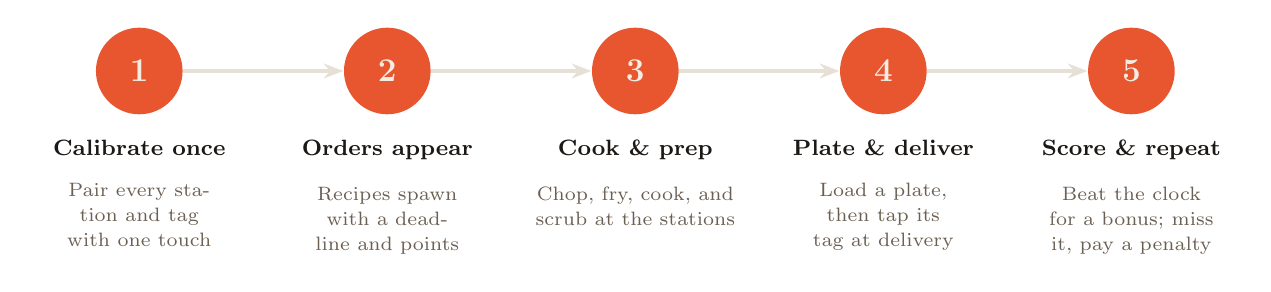
\begin{tikzpicture}[
  stepnode/.style={circle, fill=orange, text=cream, minimum size=1.1cm, font=\bfseries\large},
  lbl/.style={font=\bfseries\fontsize{8.5}{10}\selectfont, text=ink, align=center, text width=2.6cm},
  sub/.style={font=\fontsize{7}{9}\selectfont, text=mutedText, align=center, text width=2.6cm},
  arr/.style={-{Stealth[length=2.5mm]}, line width=1.2pt, draw=cardBorder}
]
\foreach \i/\name/\lbl/\sub in {
  1/n1/Calibrate once/{Pair every station and tag with one touch},
  2/n2/Orders appear/{Recipes spawn with a deadline and points},
  3/n3/Cook \& prep/{Chop, fry, cook, and scrub at the stations},
  4/n4/Plate \& deliver/{Load a plate, then tap its tag at delivery},
  5/n5/Score \& repeat/{Beat the clock for a bonus; miss it, pay a penalty}
}{
  \pgfmathsetmacro{\x}{(\i-1)*3.15}
  \node[stepnode] (c\i) at (\x,0) {\i};
  \node[lbl, below=2mm of c\i] (l\i) {\lbl};
  \node[sub, below=1mm of l\i] {\sub};
}
\foreach \i/\j in {1/2,2/3,3/4,4/5}{
  \draw[arr] (c\i.east) -- (c\j.west);
}
\end{tikzpicture}%
}

\vspace{5mm}
{\color{bodyText}\fontsize{10}{13}\selectfont
Progress lives on the server, not the station --- pick food up mid-task,
put it down on a different board of the same kind, and pick up exactly
where you left off.\par}
\end{frame}
}

% ============================================================
% 6. SYSTEM ARCHITECTURE
% ============================================================
{
\creamframe
\begin{frame}[plain]
\vspace{2mm}
\eyebrow{System Architecture}{teal}\\[2mm]
\slidetitle{Four Hops, One Source Of Truth}

\begin{center}
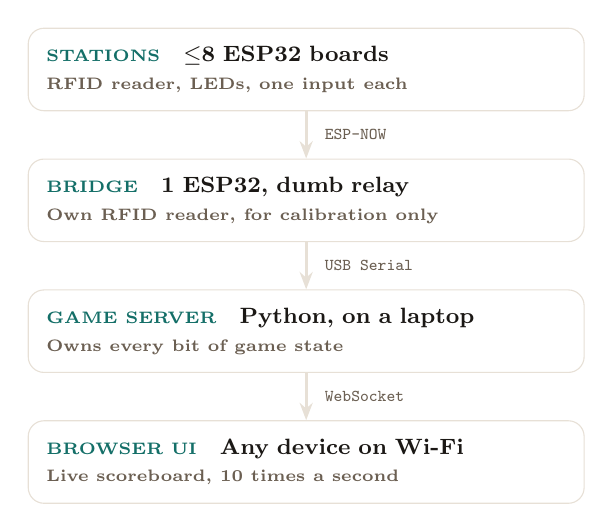
\begin{tikzpicture}[
  box/.style={draw=cardBorder, fill=white, rounded corners=2mm, align=left,
              text width=6.6cm, inner sep=2.3mm, font=\fontsize{8}{10}\selectfont},
  hop/.style={font=\ttfamily\fontsize{6.5}{8}\selectfont, text=mutedText, align=left},
  arr/.style={-{Stealth[length=2.2mm]}, line width=1.1pt, draw=cardBorder}
]
\node[box] (stations) at (0,0)
  {\color{teal}\bfseries\fontsize{6.5}{8}\selectfont STATIONS\quad{\color{ink}\bfseries\fontsize{8.5}{10}\selectfont $\le$8 ESP32 boards}\\
   {\color{mutedText} RFID reader, LEDs, one input each}};
\node[box, below=6mm of stations] (bridge)
  {\color{teal}\bfseries\fontsize{6.5}{8}\selectfont BRIDGE\quad{\color{ink}\bfseries\fontsize{8.5}{10}\selectfont 1 ESP32, dumb relay}\\
   {\color{mutedText} Own RFID reader, for calibration only}};
\node[box, below=6mm of bridge] (server)
  {\color{teal}\bfseries\fontsize{6.5}{8}\selectfont GAME SERVER\quad{\color{ink}\bfseries\fontsize{8.5}{10}\selectfont Python, on a laptop}\\
   {\color{mutedText} Owns every bit of game state}};
\node[box, below=6mm of server] (ui)
  {\color{teal}\bfseries\fontsize{6.5}{8}\selectfont BROWSER UI\quad{\color{ink}\bfseries\fontsize{8.5}{10}\selectfont Any device on Wi-Fi}\\
   {\color{mutedText} Live scoreboard, 10 times a second}};
\draw[arr] (stations.south) -- node[hop, right, xshift=1mm]{ESP-NOW} (bridge.north);
\draw[arr] (bridge.south) -- node[hop, right, xshift=1mm]{USB Serial} (server.north);
\draw[arr] (server.south) -- node[hop, right, xshift=1mm]{WebSocket} (ui.north);
\end{tikzpicture}
\end{center}

\vspace{2mm}
\begin{center}
{\color{bodyText}\itshape\fontsize{9}{12}\selectfont
Reset the round with one function call --- every station just draws what it's told.}
\end{center}
\end{frame}
}

% ============================================================
% 7. CORE PRINCIPLE
% ============================================================
{
\rustframe
\begin{frame}[plain]
\vspace{4mm}
\begin{center}
\eyebrow{Core Principle}{cream}\\[3mm]
{\color{white}\fontsize{22}{25}\selectfont\bfseries All game state lives on the laptop.}
\end{center}

\vspace{4mm}
\begin{tcolorbox}[colback=white!12!bgRust, colframe=white!35!bgRust, boxrule=0.6pt,
  arc=2mm, valign=center, coltext=white, left=3mm, right=3mm, top=1.8mm, bottom=1.8mm]
{\bfseries\fontsize{10}{12}\selectfont Tags are dumb} --- {\color{white!90!bgRust}\fontsize{9}{12}\selectfont cheap RFID chips, UID only --- never written to.}
\end{tcolorbox}
\vspace{2mm}
\begin{tcolorbox}[colback=white!12!bgRust, colframe=white!35!bgRust, boxrule=0.6pt,
  arc=2mm, valign=center, coltext=white, left=3mm, right=3mm, top=1.8mm, bottom=1.8mm]
{\bfseries\fontsize{10}{12}\selectfont Stations are dumb} --- {\color{white!90!bgRust}\fontsize{9}{12}\selectfont they report events and draw whatever they're told.}
\end{tcolorbox}
\vspace{2mm}
\begin{tcolorbox}[colback=white!12!bgRust, colframe=white!35!bgRust, boxrule=0.6pt,
  arc=2mm, valign=center, coltext=white, left=3mm, right=3mm, top=1.8mm, bottom=1.8mm]
{\bfseries\fontsize{10}{12}\selectfont The bridge is dumb} --- {\color{white!90!bgRust}\fontsize{9}{12}\selectfont just a relay between ESP-NOW and USB serial.}
\end{tcolorbox}

\vspace{5mm}
\begin{center}
{\color{white}\bfseries\fontsize{12}{15}\selectfont Reset the whole game? One function call.}
\end{center}
\end{frame}
}

% ============================================================
% 8. THE HARDWARE
% ============================================================
{
\creamframe
\begin{frame}[plain]
\vspace{2mm}
\eyebrow{The Hardware}{teal}\\[2mm]
\slidetitle{Every Station, The Same Build}

\begin{columns}[t,totalwidth=\linewidth]
\begin{column}{0.5\textwidth}
\begin{whitecard}
{\bfseries\fontsize{10}{12}\selectfont ESP32}\\[1mm]
{\color{mutedText}\fontsize{8}{10}\selectfont WiFi + ESP-NOW radio built in}
\end{whitecard}
\end{column}
\begin{column}{0.5\textwidth}
\begin{whitecard}
{\bfseries\fontsize{10}{12}\selectfont MFRC522}\\[1mm]
{\color{mutedText}\fontsize{8}{10}\selectfont Reads a tag's UID over SPI --- never writes}
\end{whitecard}
\end{column}
\end{columns}
\vspace{2mm}
\begin{columns}[t,totalwidth=\linewidth]
\begin{column}{0.5\textwidth}
\begin{whitecard}
{\bfseries\fontsize{10}{12}\selectfont WS2812B $\times$5}\\[1mm]
{\color{mutedText}\fontsize{8}{10}\selectfont One wire, addressable status LEDs}
\end{whitecard}
\end{column}
\begin{column}{0.5\textwidth}
\begin{whitecard}
{\bfseries\fontsize{10}{12}\selectfont + one input}\\[1mm]
{\color{mutedText}\fontsize{8}{10}\selectfont A limit switch, a joystick, or nothing}
\end{whitecard}
\end{column}
\end{columns}

\vspace{4mm}
\begin{columns}[t,totalwidth=\linewidth]
\begin{column}{0.33\textwidth}
\begin{darkcard}
\centering{\color{orange}\bfseries\fontsize{19}{21}\selectfont $\le$8}\\[1.8mm]
{\color{creamMuted}\fontsize{8}{10}\selectfont stations sharing one bridge}
\end{darkcard}
\end{column}
\begin{column}{0.33\textwidth}
\begin{darkcard}
\centering{\color{tealBright}\bfseries\fontsize{19}{21}\selectfont 5}\\[1.8mm]
{\color{creamMuted}\fontsize{8}{10}\selectfont LEDs per station strip}
\end{darkcard}
\end{column}
\begin{column}{0.33\textwidth}
\begin{darkcard}
\centering{\color{orange}\bfseries\fontsize{19}{21}\selectfont 32~B}\\[1.8mm]
{\color{creamMuted}\fontsize{8}{10}\selectfont max bytes in one ESP-NOW packet}
\end{darkcard}
\end{column}
\end{columns}
\end{frame}
}

% ============================================================
% 9. WHAT IT COSTS
% ============================================================
{
\creamframe
\begin{frame}[plain]
\vspace{2mm}
\eyebrow{Budget}{teal}\\[2mm]
\slidetitle{What It Costs}

\renewcommand{\arraystretch}{1.3}
{\setlength{\tabcolsep}{3pt}\fontsize{8}{10}\selectfont
\begin{tabular}{|>{\raggedright\arraybackslash}p{0.33\linewidth}|>{\raggedright\arraybackslash}p{0.15\linewidth}|>{\raggedright\arraybackslash}p{0.1\linewidth}|>{\raggedright\arraybackslash}p{0.26\linewidth}|}
\hline
\rowcolor{rowShade}\textbf{\color{mutedText}Component} & \textbf{\color{mutedText}Unit cost} & \textbf{\color{mutedText}Qty} & \textbf{\color{mutedText}Notes} \\
\hline
ESP32 dev board & \textasciitilde\$6 & 9 & 8 stations + 1 bridge \\
\hline
MFRC522 RFID reader & \textasciitilde\$2 & 9 & One per station + bridge \\
\hline
WS2812B strip (5px) & \textasciitilde\$1 & 8 & Status LEDs per station \\
\hline
Limit switch / joystick & \textasciitilde\$1.50 & 6 & Only input-driven stations \\
\hline
RFID tags (13.56 MHz) & \textasciitilde\$0.15 & 30 & Ingredients + plates \\
\hline
Wiring, perfboard, case & \textasciitilde\$4 & 9 & Rough per-station estimate \\
\hline
\end{tabular}
}

\vspace{4mm}
\begin{darkcard}
\centering{\color{orange}\bfseries\fontsize{20}{22}\selectfont \textasciitilde\$130}\\[1.5mm]
{\color{creamMuted}\fontsize{8.5}{11}\selectfont estimated total build cost for 8 stations + bridge ---
{\itshape placeholder figure, swap in your real receipts}}
\end{darkcard}
\end{frame}
}

% ============================================================
% 10. MEET THE STATIONS
% ============================================================
{
\creamframe
\begin{frame}[plain]
\vspace{1mm}
\eyebrow{Meet The Stations}{teal}\\[1.5mm]
\slidetitle{Six Jobs, One Shared Skeleton}

\begin{columns}[t,totalwidth=\linewidth]
\begin{column}{0.5\textwidth}
\begin{whitecard}
{\bfseries\fontsize{9.5}{11}\selectfont Cutting Board}\\[1mm]
{\color{teal}\bfseries\fontsize{6.5}{8}\selectfont INPUT}\ {\color{bodyText}\fontsize{7.5}{9}\selectfont Limit-switch presses}\\[0.6mm]
{\color{rustText}\bfseries\fontsize{6.5}{8}\selectfont RESULT}\ {\color{bodyText}\fontsize{7.5}{9}\selectfont Raw $\to$ Chopped}
\end{whitecard}
\vspace{1.8mm}
\begin{whitecard}
{\bfseries\fontsize{9.5}{11}\selectfont Frying Pan}\\[1mm]
{\color{teal}\bfseries\fontsize{6.5}{8}\selectfont INPUT}\ {\color{bodyText}\fontsize{7.5}{9}\selectfont Joystick: circle or zigzag}\\[0.6mm]
{\color{rustText}\bfseries\fontsize{6.5}{8}\selectfont RESULT}\ {\color{bodyText}\fontsize{7.5}{9}\selectfont Raw $\to$ Cooked}
\end{whitecard}
\vspace{1.8mm}
\begin{whitecard}
{\bfseries\fontsize{9.5}{11}\selectfont Pot}\\[1mm]
{\color{teal}\bfseries\fontsize{6.5}{8}\selectfont INPUT}\ {\color{bodyText}\fontsize{7.5}{9}\selectfont None --- timed by the server}\\[0.6mm]
{\color{rustText}\bfseries\fontsize{6.5}{8}\selectfont RESULT}\ {\color{bodyText}\fontsize{7.5}{9}\selectfont Raw $\to$ Cooked $\to$ Burnt}
\end{whitecard}
\end{column}
\begin{column}{0.5\textwidth}
\begin{whitecard}
{\bfseries\fontsize{9.5}{11}\selectfont Sink} \hfill {\scriptsize\color{white}\colorbox{tealBright}{\strut NEW}}\\[1mm]
{\color{teal}\bfseries\fontsize{6.5}{8}\selectfont INPUT}\ {\color{bodyText}\fontsize{7.5}{9}\selectfont Joystick scrubbed, any direction}\\[0.6mm]
{\color{rustText}\bfseries\fontsize{6.5}{8}\selectfont RESULT}\ {\color{bodyText}\fontsize{7.5}{9}\selectfont Configurable wash step}
\end{whitecard}
\vspace{1.8mm}
\begin{whitecard}
{\bfseries\fontsize{9.5}{11}\selectfont Plate}\\[1mm]
{\color{teal}\bfseries\fontsize{6.5}{8}\selectfont INPUT}\ {\color{bodyText}\fontsize{7.5}{9}\selectfont None --- the reader IS the plate}\\[0.6mm]
{\color{rustText}\bfseries\fontsize{6.5}{8}\selectfont RESULT}\ {\color{bodyText}\fontsize{7.5}{9}\selectfont Collects whatever's placed on it}
\end{whitecard}
\vspace{1.8mm}
\begin{whitecard}
{\bfseries\fontsize{9.5}{11}\selectfont Delivery}\\[1mm]
{\color{teal}\bfseries\fontsize{6.5}{8}\selectfont INPUT}\ {\color{bodyText}\fontsize{7.5}{9}\selectfont Touch a plate's tag here}\\[0.6mm]
{\color{rustText}\bfseries\fontsize{6.5}{8}\selectfont RESULT}\ {\color{bodyText}\fontsize{7.5}{9}\selectfont Matches an order, scores points}
\end{whitecard}
\end{column}
\end{columns}
\end{frame}
}

% ============================================================
% 11. SOFTWARE / PROTOCOL
% ============================================================
{
\creamframe
\begin{frame}[plain]
\vspace{1mm}
\eyebrow{Software $\cdot$ Protocol}{teal}\\[1.5mm]
\slidetitle{Talking Over ESP-NOW}

\begin{columns}[t,totalwidth=\linewidth]
\begin{column}{0.5\textwidth}
\begin{whitecard}
{\color{teal}\bfseries\fontsize{8}{10}\selectfont\MakeUppercase{Station $\to$ Bridge}}\\[1mm]
{\color{darkText}\fontsize{8.5}{11}\selectfont
\begin{itemize}
\item Hello, Heartbeat
\item TagPlaced, TagRemoved
\item TaskProgress, TaskDone
\end{itemize}}
\end{whitecard}
\end{column}
\begin{column}{0.5\textwidth}
\begin{whitecard}
{\color{rustText}\bfseries\fontsize{8}{10}\selectfont\MakeUppercase{Bridge $\to$ Station}}\\[1mm]
{\color{darkText}\fontsize{8.5}{11}\selectfont
\begin{itemize}
\item Welcome, Accept
\item Reject
\item SetDisplay
\end{itemize}}
\end{whitecard}
\end{column}
\end{columns}

\vspace{3mm}
\begin{center}
\tikz\node[fill=bgDark, text=cream, rounded corners=4mm, inner sep=1.5mm, font=\bfseries\fontsize{7.5}{9}\selectfont]{5$\times$ retries};
\hspace{2mm}
\tikz\node[fill=bgDark, text=cream, rounded corners=4mm, inner sep=1.5mm, font=\bfseries\fontsize{7.5}{9}\selectfont]{200ms apart};
\hspace{2mm}
{\color{mutedText}\fontsize{8}{10}\selectfont Acked and de-duplicated by (MAC, sequence) --- a lost ack never runs a handler twice.}
\end{center}

\vspace{2.5mm}
\begin{darkcard}
{\color{tealBright}\ttfamily\fontsize{8}{10}\selectfont TX AABBCCDDEEFF 6 R 02}\\
{\color{cream}\ttfamily\fontsize{8}{10}\selectfont RX AABBCCDDEEFF 2 04DEADBEEF000000000000}\\[1mm]
{\color{creamMuted}\fontsize{8}{10}\selectfont ASCII lines, hex payloads --- debuggable straight from a serial monitor.}
\end{darkcard}
\end{frame}
}

% ============================================================
% 12. SOFTWARE / GAME SERVER
% ============================================================
{
\creamframe
\begin{frame}[plain]
\vspace{2mm}
\eyebrow{Software $\cdot$ Game Server}{teal}\\[1.5mm]
\slidetitle{The Server Owns Every Bit Of State}

\begin{columns}[t,totalwidth=\linewidth]
\begin{column}{0.5\textwidth}
\begin{whitecard}
{\bfseries\fontsize{10}{12}\selectfont Pure Engine}\\[1mm]
{\color{bodyText}\fontsize{8.5}{11}\selectfont A single class runs on events, a tick, and an injectable clock --- no serial or network inside, so tests drive it with fake time.}
\end{whitecard}
\vspace{2mm}
\begin{whitecard}
{\bfseries\fontsize{10}{12}\selectfont Calibration Wizard}\\[1mm]
{\color{bodyText}\fontsize{8.5}{11}\selectfont Touch any tag to the bridge to name it, touch it to every station, then touch each ingredient once. Saved to disk, reloadable.}
\end{whitecard}
\end{column}
\begin{column}{0.5\textwidth}
\begin{whitecard}
{\bfseries\fontsize{10}{12}\selectfont One Behaviour Per Kind}\\[1mm]
{\color{bodyText}\fontsize{8.5}{11}\selectfont A small class per station kind decides the rules; the numbers live in a level file, not in code.}
\end{whitecard}
\vspace{2mm}
\begin{whitecard}
{\bfseries\fontsize{10}{12}\selectfont Live Web UI}\\[1mm]
{\color{bodyText}\fontsize{8.5}{11}\selectfont Pushes the full game state over a websocket, ten times a second, to a plain-JavaScript scoreboard --- no build step.}
\end{whitecard}
\end{column}
\end{columns}
\end{frame}
}

% ============================================================
% 13. ENGINEERING RIGOR
% ============================================================
{
\creamframe
\begin{frame}[plain]
\vspace{0.5mm}
\eyebrow{Engineering Rigor}{teal}\\[0.8mm]
\slidetitle{Built To Survive Contact With Real Hardware}

\begin{whitecard}[top=1mm,bottom=1mm]
{\bfseries\fontsize{9}{11}\selectfont One Source Of Truth} --- {\color{bodyText}\fontsize{8}{10}\selectfont a test parses the C++ header and fails the build the moment Python's protocol drifts from the firmware.}
\end{whitecard}
\vspace{0.7mm}
\begin{whitecard}[top=1mm,bottom=1mm]
{\bfseries\fontsize{9}{11}\selectfont Zero-Hardware Dev} --- {\color{bodyText}\fontsize{8}{10}\selectfont a simulated bridge speaks the real line protocol --- the whole game runs with zero boards plugged in.}
\end{whitecard}
\vspace{0.7mm}
\begin{whitecard}[top=1mm,bottom=1mm]
{\bfseries\fontsize{9}{11}\selectfont Tested End To End} --- {\color{bodyText}\fontsize{8}{10}\selectfont Python tests plus native C++ unit tests for each station's pure logic --- no ESP32 required.}
\end{whitecard}

\vspace{2mm}
\begin{columns}[t,totalwidth=\linewidth]
\begin{column}{0.33\textwidth}
\begin{darkcard}[top=1.2mm,bottom=1.2mm]
\centering{\color{orange}\bfseries\fontsize{16}{18}\selectfont 102}\\[1.2mm]
{\color{creamMuted}\fontsize{7.5}{9}\selectfont Python tests, sub-second}
\end{darkcard}
\end{column}
\begin{column}{0.33\textwidth}
\begin{darkcard}[top=1.2mm,bottom=1.2mm]
\centering{\color{tealBright}\bfseries\fontsize{16}{18}\selectfont 21}\\[1.2mm]
{\color{creamMuted}\fontsize{7.5}{9}\selectfont native C++ tests, three firmware projects}
\end{darkcard}
\end{column}
\begin{column}{0.33\textwidth}
\begin{darkcard}[top=1.2mm,bottom=1.2mm]
\centering{\color{orange}\bfseries\fontsize{16}{18}\selectfont 0}\\[1.2mm]
{\color{creamMuted}\fontsize{7.5}{9}\selectfont boards needed to run any of them}
\end{darkcard}
\end{column}
\end{columns}
\end{frame}
}

% ============================================================
% 14. WHAT'S NEXT
% ============================================================
{
\creamframe
\begin{frame}[plain]
\vspace{2mm}
\eyebrow{What's Next}{teal}\\[1.5mm]
\slidetitle{What's Cooking Next}

\renewcommand{\arraystretch}{1.5}
{\fontsize{9.5}{12}\selectfont
\begin{tabular}{@{}p{0.09\linewidth}p{0.86\linewidth}@{}}
{\color{orange}\bfseries\fontsize{12}{14}\selectfont 01} &
\textbf{Tune on real hardware} --- RC522 removal timing, joystick dead zone, cook times \\ \hline
{\color{orange}\bfseries\fontsize{12}{14}\selectfont 02} &
\textbf{Give the sink a real recipe} --- it's wired end to end, but no ingredient uses it yet \\ \hline
{\color{orange}\bfseries\fontsize{12}{14}\selectfont 03} &
\textbf{Show plate contents on their LEDs} --- one more display mode, mirrored on both sides \\ \hline
{\color{orange}\bfseries\fontsize{12}{14}\selectfont 04} &
\textbf{Read more than one tag at once} --- several foods on a single plate, via RC522 anticollision \\ \hline
{\color{orange}\bfseries\fontsize{12}{14}\selectfont 05} &
\textbf{Watch bridge health} --- catch a hung-but-connected bridge, not just a disconnected one \\
\end{tabular}
}
\end{frame}
}

% ============================================================
% 15. THE TEAM
% ============================================================
{
\creamframe
\begin{frame}[plain]
\vspace{2mm}
\eyebrow{Credits}{teal}\\[2mm]
\slidetitle{The Team}

\begin{columns}[t,totalwidth=\linewidth]
\begin{column}{0.25\textwidth}
\centering
\avatarplaceholder[1.6cm]{PHOTO}\\[2mm]
{\bfseries\fontsize{9.5}{11}\selectfont [Name]}\\
{\color{mutedText}\fontsize{7.5}{9}\selectfont Firmware \& Stations}
\end{column}
\begin{column}{0.25\textwidth}
\centering
\avatarplaceholder[1.6cm]{PHOTO}\\[2mm]
{\bfseries\fontsize{9.5}{11}\selectfont [Name]}\\
{\color{mutedText}\fontsize{7.5}{9}\selectfont Game Server \& Protocol}
\end{column}
\begin{column}{0.25\textwidth}
\centering
\avatarplaceholder[1.6cm]{PHOTO}\\[2mm]
{\bfseries\fontsize{9.5}{11}\selectfont [Name]}\\
{\color{mutedText}\fontsize{7.5}{9}\selectfont Hardware \& Wiring}
\end{column}
\begin{column}{0.25\textwidth}
\centering
\avatarplaceholder[1.6cm]{PHOTO}\\[2mm]
{\bfseries\fontsize{9.5}{11}\selectfont [Name]}\\
{\color{mutedText}\fontsize{7.5}{9}\selectfont UI \& Product}
\end{column}
\end{columns}

\vspace{8mm}
\begin{center}
{\color{mutedText}\itshape\fontsize{9}{12}\selectfont [Add names, roles, and GitHub / contact links before presenting.]}
\end{center}
\end{frame}
}

% ============================================================
% 16. CLOSING
% ============================================================
{
\darkframe
\begin{frame}[plain]
\begin{tikzpicture}[remember picture, overlay]
  \clip (current page.south west) rectangle ($(current page.north east)+(-\videostripw-\videostripgap,0)$);
  \fill[tealBright, opacity=0.14] ([xshift=-1.2cm,yshift=-1.4cm]current page.north east) circle (2.4cm);
  \fill[orange, opacity=0.12] ([xshift=-3.2cm,yshift=1.4cm]current page.south east) circle (1.7cm);
\end{tikzpicture}
\vspace{10mm}
\eyebrow{Thank You}{orange}\\[5mm]
{\color{cream}\fontsize{34}{38}\selectfont\bfseries Come Break It.}\\[5mm]
\begin{minipage}{0.82\linewidth}
{\color{creamMuted}\fontsize{12}{17}\selectfont
Jam the joystick, yank a tag mid-chop, unplug the bridge mid-round --- the
server is built to shrug it off and pick up right where you left it.\par}
\end{minipage}
\vfill
\begin{flushleft}
{\color{creamMuted}\ttfamily\footnotesize undercooked-irl}
\end{flushleft}
\vspace{-8mm}
\hfill{\color{creamMuted}\footnotesize [Names / contact]}
\end{frame}
}

\end{document}
